\documentclass[tikz,border=4pt]{standalone}
% Shared look for the per-pattern diagrams. Copied from the IATEFL LTSIG talk
% (talks/doubly-personalised-language-learning/figures/llm-patterns.tex).
\usepackage{amssymb}
\usepackage{fontspec}
\setmainfont{Helvetica Neue}
\usetikzlibrary{arrows.meta,positioning,calc,fit}
\definecolor{ink}{HTML}{23373B}
\definecolor{hlc}{HTML}{C2410C}
\definecolor{okc}{HTML}{2E7D32}
\definecolor{badc}{HTML}{B91C1C}
\tikzset{
  mini/.style={rounded corners=2pt, minimum height=7mm, align=center,
               font=\small\color{ink}, fill=white, draw=ink!70, line width=0.6pt, inner sep=3pt},
  minillm/.style={mini, fill=hlc, draw=hlc, font=\small\bfseries\color{white}},
  fixed/.style={mini, fill=ink!12},                 % the fixed part of a prompt
  sarr/.style={-{Stealth[length=2mm]}, ink, line width=0.8pt},
  lbl/.style={font=\footnotesize\itshape\color{ink!75}},
  ok/.style={font=\small\bfseries\color{okc}},
  bad/.style={font=\small\bfseries\color{badc}},
}

% LLM Output Provenance, the problem in Zeeguu: audio lessons as stored until
% August 2026. Every row carries the same created_by label, whatever prompt
% wrote it, so the rows with the ambiguous question (red) cannot be told apart
% by a query. Real rows from audio_lesson_meaning (ids 955, 3629, 4150, 37973).
% A table, not a flow: no arrows.
\begin{document}
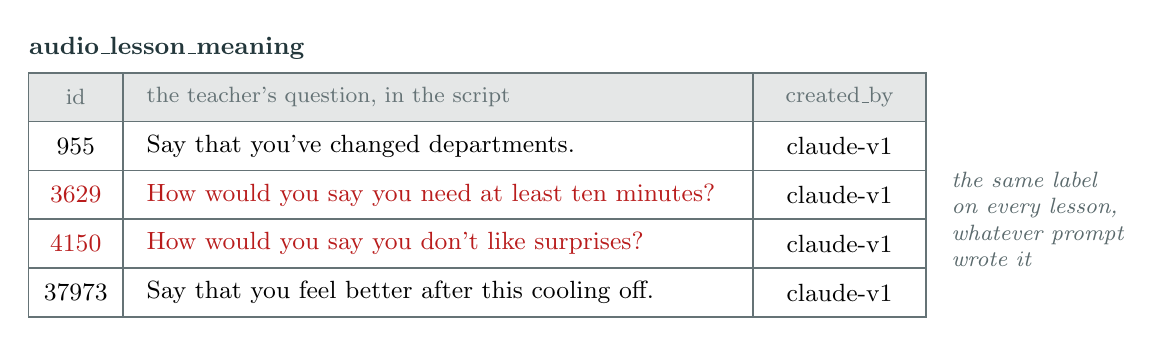
\begin{tikzpicture}[
  cell/.style={mini, rounded corners=0pt, minimum height=6.2mm, inner ysep=1pt, inner xsep=3pt, font=\small},
  head/.style={fill=ink!12, font=\footnotesize, text=ink!70},
  badrow/.style={text=badc},
  tname/.style={font=\small\bfseries, text=ink}]
\node[tname, anchor=south west, inner xsep=0pt] at (0.00,0.05) {audio\_lesson\_meaning};
\node[cell, head, minimum width=12mm] at (0.600,-0.310) {id};
\node[cell, minimum width=12mm] at (0.600,-0.930) {955};
\node[cell, minimum width=12mm, badrow] at (0.600,-1.550) {3629};
\node[cell, minimum width=12mm, badrow] at (0.600,-2.170) {4150};
\node[cell, minimum width=12mm] at (0.600,-2.790) {37973};
\node[cell, head, minimum width=80mm, text width=74mm, align=left] at (5.200,-0.310) {the teacher's question, in the script};
\node[cell, minimum width=80mm, text width=74mm, align=left] at (5.200,-0.930) {Say that you've changed departments.};
\node[cell, minimum width=80mm, text width=74mm, align=left, badrow] at (5.200,-1.550) {How would you say you need at least ten minutes?};
\node[cell, minimum width=80mm, text width=74mm, align=left, badrow] at (5.200,-2.170) {How would you say you don't like surprises?};
\node[cell, minimum width=80mm, text width=74mm, align=left] at (5.200,-2.790) {Say that you feel better after this cooling off.};
\node[cell, head, minimum width=22mm] (H) at (10.300,-0.310) {created\_by};
\node[cell, minimum width=22mm] (C0) at (10.300,-0.930) {claude-v1};
\node[cell, minimum width=22mm] at (10.300,-1.550) {claude-v1};
\node[cell, minimum width=22mm] at (10.300,-2.170) {claude-v1};
\node[cell, minimum width=22mm] (C3) at (10.300,-2.790) {claude-v1};
\node[lbl, align=left, anchor=west] at (11.600,-1.860) {the same label\\on every lesson,\\whatever prompt\\wrote it};
\end{tikzpicture}
\end{document}
